\documentclass{article}
\usepackage{cmap}
\usepackage[utf8]{inputenc}
\usepackage[english,ukrainian]{babel}
\usepackage{graphicx}
\usepackage{geometry}
\usepackage{listings}
\usepackage{float}
\usepackage{amsmath}
\geometry{
	a4paper,
	left=20mm,
	right=20mm,
	top=15mm,
	bottom=15mm,
}
\lstset{
	language=c,
	tabsize=4,
	keepspaces,
	showstringspaces=false,
}
\graphicspath{ {./pictures} }
\setlength{\parindent}{4em}

\newcommand\subject{Основи електроніки}
\newcommand\lecturer{професор кафедри ПЗ \\ Фечан А.В.}
\newcommand\teacher{доцент кафедри ПЗ \\ Коцун В.І.}
\newcommand\mygroup{ПЗ-22}
\newcommand\lab{5}
\newcommand\theme{Дослідження роботи підсилювачів змінного струму}
\newcommand\purpose{Засвоїти методи розрахунку елементів схем підсилювачів,
	ознайомитись зі схемами багато каскадних підсилювачів}

\begin{document}
\begin{normalsize}
	\begin{titlepage}
		\thispagestyle{empty}
		\begin{center}
			\textbf{МІНІСТЕРСТВО ОСВІТИ І НАУКИ УКРАЇНИ\\
				НАЦІОНАЛЬНИЙ УНІВЕРСИТЕТ "ЛЬВІВСЬКА ПОЛІТЕХНІКА"}
		\end{center}
		\begin{flushright}
			\textbf{ІКНІ}\\
			Кафедра \textbf{ПЗ}
		\end{flushright}
		\vspace{200pt}
		\begin{center}
			\textbf{ЗВІТ}\\
			\vspace{10pt}
			до лабораторної роботи № \lab\\
			\textbf{на тему}: “\textit{\theme}”\\
			\textbf{з дисципліни}: “\subject”
		\end{center}
		\vspace{112pt}
		\begin{flushright}
			
			\textbf{Лектор}:\\
			\lecturer\\
			\vspace{28pt}
			\textbf{Виконав}:\\
			
			студент групи \mygroup\\
			Коваленко Д.М.\\
			\vspace{28pt}
			\textbf{Прийняв}:\\
			
			\teacher\\
			
			\vspace{28pt}
			«\rule{1cm}{0.15mm}» \rule{1.5cm}{0.15mm} 2023 р.\\
			$\sum$ = \rule{1cm}{0.15mm}……………\\
			
		\end{flushright}
		\vspace{\fill}
		\begin{center}
			\textbf{Львів — 2023}
		\end{center}
	\end{titlepage}
		
	\begin{description}
		\item[Тема.] \theme.
		\item[Мета.] \purpose.
	\end{description}

	\section*{Теоретичні відомості}
	Часто виникає потреба переводити слабкий вхідний електричний сигнал (від електромагнітного поля, різного роду датчиків) на вищий енергетичний рівень, де його зможуть сприйняти різного виду виконавчі пристрої або органи чуття живих організмів. 
	
	Найбільш поширений спосіб такого підсилення ґрунтується на тому, що вхідний електричний сигнал uвх за допомогою керуючого елемента КЕ впливає на роботу джерела електричної енергії (джерело живлення Еж), відтворюючись завдяки цьому на вищому енергетичному рівні (рис.1). Якщо керуючий елемент КЕ побудовано на базі електронного приладу, то таке підсилення називають електронним. 
	
	Принцип електронного підсилення полягає у перетворенні енергії джерела постійної напруги Еж в енергію змінного вихідного сигналу uвих шляхом зміни провідності КЕ за законом, зумовленим формою вхідного сигналу uвх. Основою електронного підсилювача є підсилювальний каскад, який в якості керуючого елемента має біполярний або польовий транзистор. Він характеризується коефіцієнтами підсилення, що визначаються відношеннями вихідних параметрів до вхідних.

	Залежно від того, який параметр домінує, розрізняють підсилювальні каскади за напругою, струмом і потужністю. Структурна схема підсилювального каскаду.
	
	Якщо забезпечити потрібне підсилення одним каскадом неможливо, то його вихідний сигнал можна подати як вхідний на наступний каскад, і так далі, доки не буде досягнуто необхідного коефіцієнта підсилення. У такий спосіб створюють багатокаскадний підсилювач.
	
	За видом зв’язку між джерелом сигналу, каскадами та навантаженням підсилювачі поділяються на підсилювачі з безпосереднім, резистивним, оптронним, резистивно-ємнісним, трансформаторним або резонансно-трансформаторним зв’язком.
	
	\section*{Індивідуальне завдання}
	\begin{enumerate}
		\item Складіть схему, наведену на рис. 1 в пакеті Multisim, яка дозволяє досліджувати однокаскадний підсилювач на біполярних транзисторах. Встановіть в схемі розрахункове значення Rb2*; значення опорів резисторів Rb1, Rb2, Rb3 прийняти рівними відповідно 0,8·Rb1* , Rb1* , 1,2·Rb1* .
		
		\item Подайте на вхід підсилювача синусоїдальну напругу Uвх m = 10 mV, F = 1 kHz і для кожного з опорів Rb1, Rb2, Rb3 зняти осцилограми вхідної та вихідної напруг (точки 1, 2, 3). Поясніть отримані осцилограми.
		
		\item Активізуйте аналізатор частотних характеристик і зніміть залежність коефіцієнта підсилювання КU від частоти вхідного сигналу F при Rb2, що дорівнює розрахунковому Rb1* та фазовий зсув Uвих відносно Uвх. Заповнити таблицю 11.1 (8÷10 значень F в робочому діапазоні).
		
		\item Збільшіть в два рази значення перехідних ємностей Сd1 і Cd2 та зменшити в два рази значення «паразитної» ємності Ср. Повторіть п. 2.3. Поясніть зміни в залежностях KU(F) і f(F), побудувавши їх на одному графіку. 
		Визначіть смугу підсилення на рівні 0,707К0, де К0 – середнє значення KU в середині робочого діапазону.
		
		\item Складіть схему, наведену на рис. 2, яка дозволяє досліджувати підсилювач на польовому транзисторі.
		
		\item Для двох значень Rd (3,5 kOhm та 7,0 kOhm) отримайте осцилограми Uвх(t) і Uвих(t), визначіть  і зробіть висновок щодо впливу Rd на KU. Поясніть роль опору R3, що є в колі витоку «s». Параметри вхідного сигналу, які необхідно встановити на генераторі: Uвх m = 50 mV, F = 1 kHz.
		
		\item Складіть схему, наведену на рис. 3, яка дозволяє проводити дослідження двокаскадного підсилювача на транзисторах. Поясніть призначення кожного елемента схеми.
		
		\item Подайте на вхід синусоїдальний сигнал Uвх m = 10 mV, F = 1 kHz. Зніміть осцилограми вхідної та вихідної напруги Uвих m 1 для першого каскаду підсилення (токи 1, 2), потім для двох каскадів Uвих m 2 (токи 1, 3). Визначіть KU 1 та KU заг. Доведіть, що KU заг = KU 1· KU 2.
		
		\item Спираючись на показання приладів в схемі на рис. 5, визначіть значення якого з елементів схеми слід змінити, щоб забезпечити роботу підсилювача на середині лінійного діапазону (в класі А).
	\end{enumerate}

	\section*{Хід виконання}
	
	\begin{figure}[H]
		\centering
		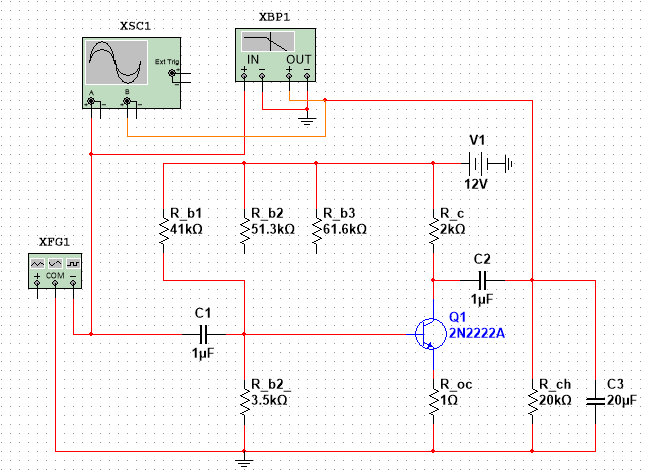
\includegraphics[width=\textwidth]{1}
		\caption{Схема 1}
	\end{figure}

	\begin{figure}[H]
		\centering
		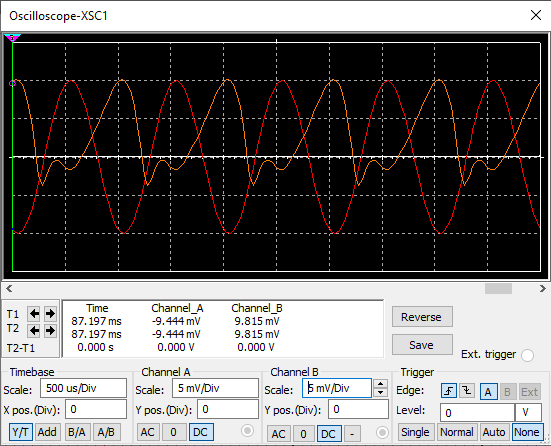
\includegraphics[width=\textwidth]{11}
		\caption{Осцилограма для опору 41к Ом}
	\end{figure}

	\begin{figure}[H]
		\centering
		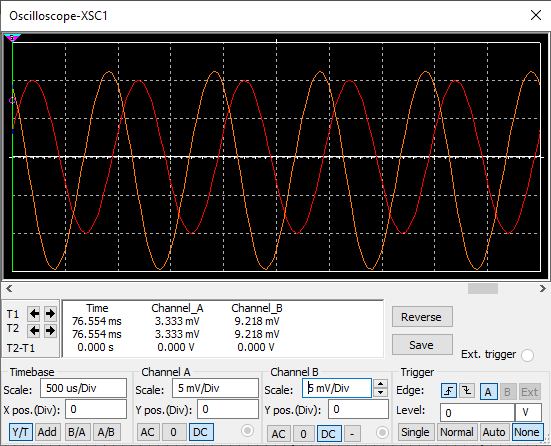
\includegraphics[width=\textwidth]{12}
		\caption{Осцилограма для опору 51.3к Ом}
	\end{figure}
	
	\begin{figure}[H]
		\centering
		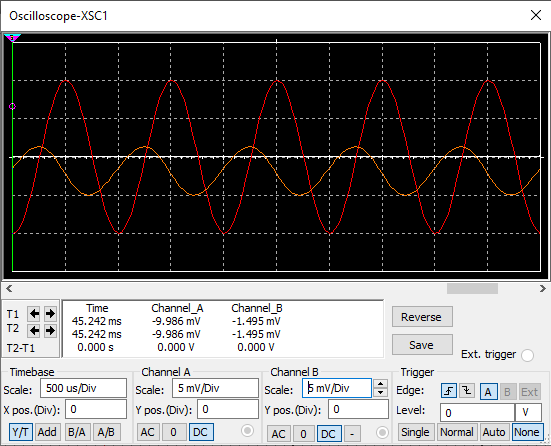
\includegraphics[width=\textwidth]{13}
		\caption{Осцилограма для опору 61.6к Ом}
	\end{figure}
	
	\begin{figure}[H]
		\centering
		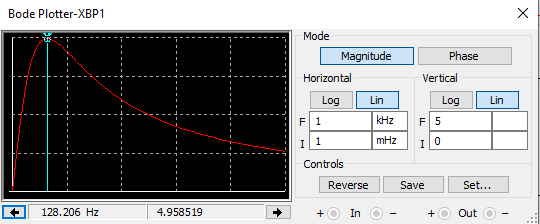
\includegraphics[width=\textwidth]{14}
		\caption{Отримана залежність коефіцієнта підсилювання від частоти}
	\end{figure}
	
	\begin{figure}[H]
		\centering
		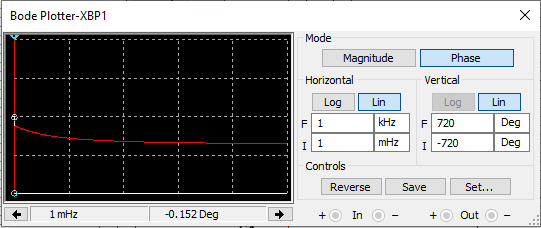
\includegraphics[width=\textwidth]{15}
		\caption{Отримана залежність фазового зсуву від частоти}
	\end{figure}
	
	\begin{table}[H]
		\centering
		\renewcommand*\arraystretch{1.3}
		\begin{tabular}{|p{0.12\linewidth}|p{0.08\linewidth}|p{0.08\linewidth}|p{0.08\linewidth}|p{0.08\linewidth}|p{0.08\linewidth}|p{0.08\linewidth}|p{0.08\linewidth}|p{0.08\linewidth}|}
			\hline
			$F$, $Hz$&25&50&75&100&250&500&750&1000\\
			\hline
			$K_U$&2.0&3.3&4.3&4.8&4.1&2.5&1.7&1.3\\
			\hline
			Ф, град&-113&-132&-151&-166&-214&-240&-249&-254\\
			\hline
		\end{tabular}
		\caption{Отримана таблиця}
	\end{table}
	
	\begin{table}[H]
		\centering
		\renewcommand*\arraystretch{1.3}
		\begin{tabular}{|p{0.12\linewidth}|p{0.08\linewidth}|p{0.08\linewidth}|p{0.08\linewidth}|p{0.08\linewidth}|p{0.08\linewidth}|p{0.08\linewidth}|p{0.08\linewidth}|p{0.08\linewidth}|}
			\hline
			$F$, $Hz$&25&50&75&100&250&500&750&1000\\
			\hline
			$K_U$&12.9&17.8&18.8&17.7&9.8&5.2&3.5&2.6\\
			\hline
			Ф, град&-131&-160&-183&-200&-238&-253&-259&-261\\
			\hline
		\end{tabular}
		\caption{Отримана таблиця при збільшенні перехідних ємностей в 2 рази та зменшення "паразитної" ємності в 2 рази}
	\end{table}
	
	\begin{figure}[H]
		\centering
		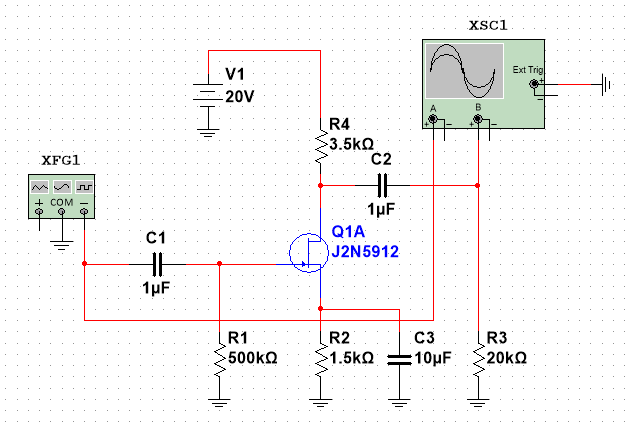
\includegraphics[width=\textwidth]{2}
		\caption{Схема 2}
	\end{figure}
	
	\begin{figure}[H]
		\centering
		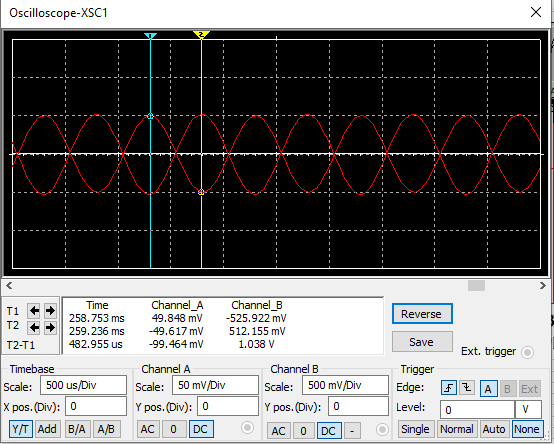
\includegraphics[width=\textwidth]{21}
		\caption{Осцилограма при опорі $R_d$ = $3.5$к Ом, $K_U$ = $512/50=10.2$}
	\end{figure}
	
	\begin{figure}[H]
		\centering
		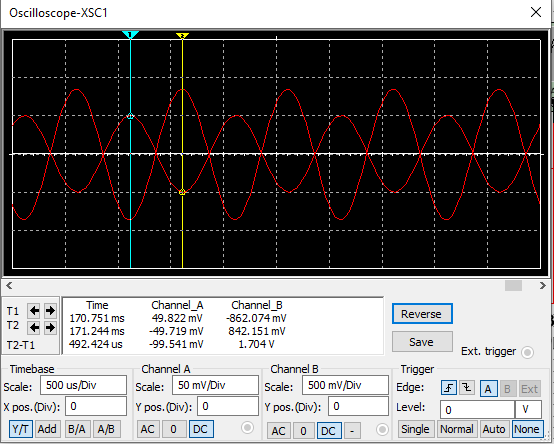
\includegraphics[width=\textwidth]{22}
		\caption{Осцилограма при опорі $R_d$ = $7$к Ом, $K_U = 840/50= 16.8$}
	\end{figure}
	
	Отже, із збільшенням опору $R_d$ коефіцієнт підсилення збільшився.	Опір $R_3$, як і конденсатор поряд необхідний для компенсації температурного зсуву.
	
	\begin{figure}[H]
		\centering
		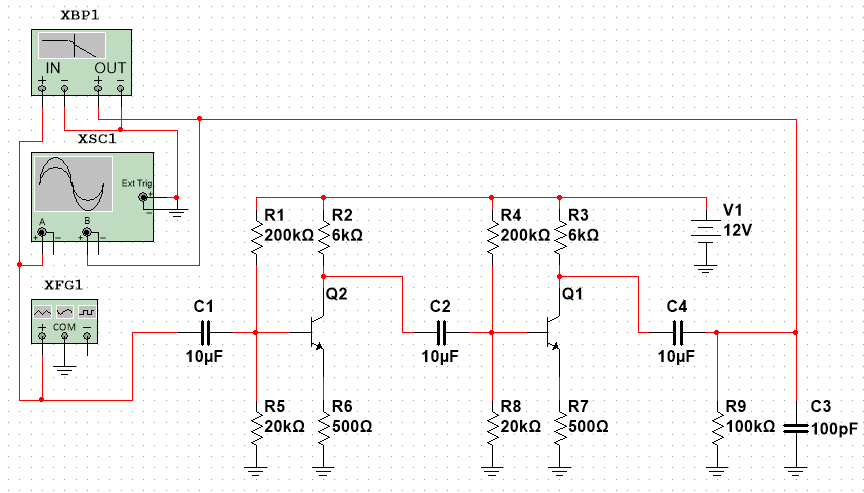
\includegraphics[width=\textwidth]{3}
		\caption{Схема 3}
	\end{figure}
	
	\begin{figure}[H]
		\centering
		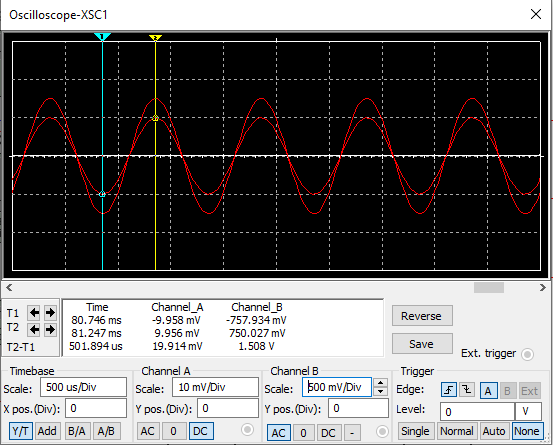
\includegraphics[width=\textwidth]{31}
		\caption{Осцилограма для двох каскадів (точки 1 і 3), $K_{U\text{заг}} = 750/10= 75$}
	\end{figure}
	
	\begin{figure}[H]
		\centering
		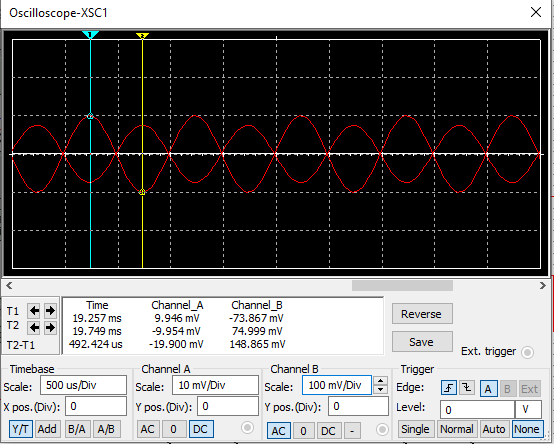
\includegraphics[width=\textwidth]{32}
		\caption{Осцилограма для першого каскаду (точки 1 і 2), $K_{U1} = 75/10= 7.5$}
	\end{figure}
	
	З отриманих коефіцієнтів отримуємо, що $K_{U2} = K_{U\text{заг}} / K_{U1} = 75 / 7.5= 10$
	З іншого боку, за отриманими показниками напруг $K_{U2} = 750 / 75 = 10$
	Отже, $К_U\text{заг}$ справді дорівнює добутку $К_{U1}$ на $К_{U2}$.
	
	\begin{figure}[H]
		\centering
		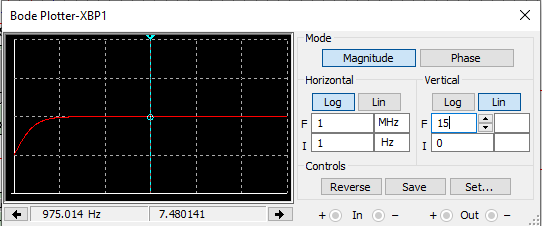
\includegraphics[width=\textwidth]{33}
		\caption{Коефіцієнт підсилення для першого каскаду (точки 1 і 2)}
	\end{figure}
	
	\begin{figure}[H]
		\centering
		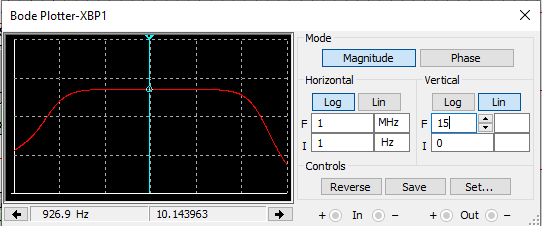
\includegraphics[width=\textwidth]{34}
		\caption{Коефіцієнт підсилення для другого каскаду (точки 2 і 3)}
	\end{figure}
	
	\begin{figure}[H]
		\centering
		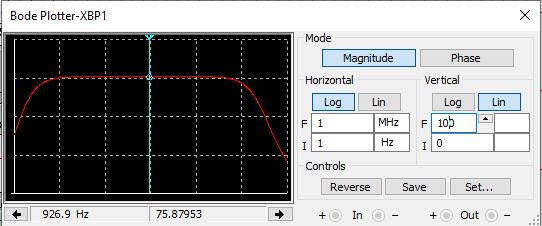
\includegraphics[width=\textwidth]{35}
		\caption{Коефіцієнт підсилення для двох каскадів (точки 1 і 3)}
	\end{figure}
	
	\section*{Висновки}
	Під час виконання лабораторної роботи я ознайомився із схемами підсилювачів на біполярних і польових транзисторах, багатокаскадними підсилювачами, дослідив відповідні схеми в Multisim, обрахував коефіцієнти підсилення та їх залежність від інших характеристик схеми, пояснив призначення кожного елемента в схемах.
	    
\end{normalsize}
\end{document}
